\documentclass[11pt,a4paper]{article}
\usepackage[margin=2.4cm]{geometry}
\usepackage[T1]{fontenc}
\usepackage{lmodern}
\usepackage{microtype}
\usepackage{amsmath,amssymb}
\usepackage{graphicx}
\usepackage{xcolor}
\usepackage{booktabs}
\usepackage{tikz}
\usetikzlibrary{decorations.pathmorphing,arrows.meta}
\usepackage{caption}
\captionsetup{font=small,labelfont=bf}
\usepackage[breaklinks=true]{hyperref}
\hypersetup{colorlinks=true,linkcolor=blue!60!black,urlcolor=blue!55!black}

\newcommand{\warn}[1]{\par\noindent\colorbox{red!8}{\parbox{\dimexpr\linewidth-2\fboxsep}{#1}}\par}

\title{\textbf{A tunable weak-field applicator for testing radical-pair
ROS modulation in exercise recovery}\\[4pt]
\large Build specification and self-controlled experimental protocol}
\author{O.~Kirichenko\\[2pt]\small
  \href{mailto:urevich55@gmail.com}{urevich55@gmail.com}}
\date{\today}

\begin{document}
\maketitle

\warn{\textbf{Read first — status and safety.} This is a
\emph{research instrument}, not a medical device or a treatment. It is
built to \emph{measure} whether a weak magnetic field changes recovery
markers, not to deliver a promised benefit. Static fields up to 3~mT are
$\sim\!60\times$ Earth's field and far below a fridge magnet or MRI, with
no established acute hazard; nonetheless, do not use with any implanted
electronic device (pacemaker, pump), and any protocol on other people
requires ethics oversight. The predicted effect is a \emph{few percent}
and unproven in living humans. Crucially, suppressing exercise ROS is
\textbf{not} automatically beneficial (Sec.~\ref{sec:hormesis}).}

\section{Purpose}
The companion note~\cite{cisspaper} models the mitochondrial
flavin--superoxide radical pair as a spin gate whose triplet
(superoxide-escape) yield depends on a weak applied magnetic field, on the
scale of the flavin hyperfine coupling ($\sim\!0.2$--$3$~mT). Usselman
et~al.~\cite{usselman} measured exactly such a millitesla-scale shift in
the cellular $\text{O}_2^{\bullet-}/\text{H}_2\text{O}_2$ ratio. This
document specifies a low-cost apparatus that produces a \emph{tunable,
uniform} field over a limb, and a \emph{sham-controlled} protocol to test
whether scanning that field measurably affects post-exercise recovery.

\section{Field applicator (Helmholtz pair)}
A Helmholtz pair gives a uniform field over a central region large enough
for a forearm or calf. With coil radius $R$ and coil separation equal to
$R$, the central field is
\begin{equation}
  B = \left(\tfrac{4}{5}\right)^{3/2}\frac{\mu_0 N I}{R}.
\end{equation}
For $R=0.15$~m (30~cm coils, 15~cm apart) the uniform region is
$\sim\!9$~cm across. Table~\ref{tab:coil} gives the current for each
target field at $N=100$ turns per coil.

\begin{table}[h]
\centering
\begin{tabular}{lrr}
\toprule
target $B$ & ampere-turns $NI$ & current $I$ ($N{=}100$)\\
\midrule
0.2 mT (near the effect peak) & 33 & 0.33 A\\
1.0 mT & 167 & 1.67 A\\
3.0 mT (upper scan) & 500 & 5.00 A\\
\bottomrule
\end{tabular}
\caption{Helmholtz drive currents, $R=0.15$~m.}
\label{tab:coil}
\end{table}

\noindent\textbf{Concrete build.} Two coils of $N=100$ turns of AWG20
(0.5~mm$^2$) enamelled copper on 30~cm formers. Wire length $\approx188$~m,
coil-pair resistance $\approx6.3~\Omega$. At the 3~mT maximum the pair
dissipates $\approx160$~W; a typical protocol runs at $\le1$~mT
($\approx20$~W) from a 12~V supply. \textbf{Drive:} a constant-current
source (a buck/linear current regulator; the UC3843-class controller from
common maker kits works) with a front-panel set-point for $B$. Keep the
duty modest and let the coils warm-limit; add an NTC cutout at 45\,$^\circ$C.

\section{Calibration}
Do not trust the set-point dial---\emph{measure} the field. A Hall-effect
gaussmeter or a calibrated linear Hall sensor (e.g. a $\pm10$~mT ratiometric
sensor) at the limb position maps current to $B$ before any session. This
step is what separated the honest instruments from the folklore devices in
the wider ``energy'' literature: the number on the coil must be verified,
not assumed.

\section{Dose plan}
Figure~\ref{fig:dose} shows the model's predicted change in superoxide
versus field, with recommended set-points to scan: $0$ (sham/off),
$0.2$, $0.5$, $1.0$ and $3.0$~mT. The predicted signal is largest near the
$0.2$--$0.5$~mT resonance and declines toward $3$~mT---so the experiment
should concentrate points at low field, not high.

\begin{figure}[h]
\centering
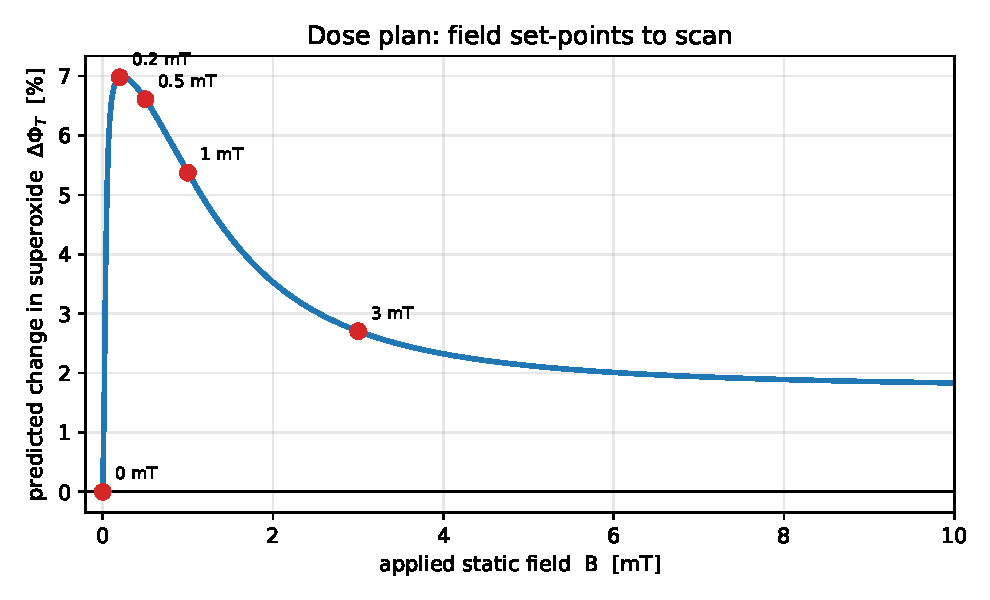
\includegraphics[width=0.66\textwidth]{fig_dose_plan.pdf}
\caption{Predicted change in superoxide yield $\Delta\Phi_T$ vs applied
field (radical-pair model, CISS $P=0.35$); red points are the recommended
experimental set-points. The effect peaks near $0.2$--$0.5$~mT.}
\label{fig:dose}
\end{figure}

\section{Sham-controlled self-experiment}
The single most important design element is a \textbf{sham coil} that looks,
sounds and warms identically but produces no net field (bifilar/counter-wound
so the currents cancel). Sessions are \textbf{blinded} (a helper sets
real/sham from a coded list; you do not know which) and \textbf{crossed
over} (each condition repeated on matched days).

\medskip\noindent\textbf{Recovery read-outs} (choose $\ge2$; all
low-cost, non-invasive):
\begin{itemize}\itemsep2pt
\item \textbf{HRV} (heart-rate variability, rMSSD) each morning from a
  chest strap or ring---the cleanest daily recovery proxy;
\item \textbf{perceived soreness} (DOMS) on a 0--10 scale at $+24$ and
  $+48$~h;
\item \textbf{force recovery}: countermovement-jump height or grip
  dynamometer at $+24/+48$~h vs pre-exercise;
\item optional \textbf{creatine kinase} (finger-prick point-of-care) as a
  muscle-damage marker.
\end{itemize}

\medskip\noindent\textbf{Session flow (one condition):} standardized run
$\rightarrow$ apply coil to the worked limb for 30--60~min at the assigned
$B$ (or sham) $\rightarrow$ log read-outs at $+24$ and $+48$~h. Repeat each
condition $\ge5$ times before comparing; a real few-percent physiological
effect needs $\sim$dozens of paired sessions to clear day-to-day noise,
which is the honest cost of measuring something this small.

\medskip\noindent\textbf{Analysis:} paired comparison (real vs sham) per
read-out; treat $B$ as the dose axis of Fig.~\ref{fig:dose}. A genuine
effect appears as a \emph{dose-shaped} response peaking at low field, not a
flat offset (which would flag a placebo or a thermal artifact from the
coil warming the limb---control for that with the sham's matched heat).

\section{The bifilar sham coil}
\label{sec:sham}
The sham must be electrically and thermally identical to the real coil but
produce \emph{no net field}. This is achieved by winding it
\textbf{bifilar}: two enamelled wires laid side by side and wound together
as one, then connected so that the current runs \emph{out} along wire~1 and
\emph{back} along wire~2. Every turn then carries $+I$ and $-I$ a
millimetre apart, so the magnetic fields cancel to $<1\%$ of the real coil,
while the wire length, resistance and ohmic heating are the same
(Fig.~\ref{fig:bifilar}). Use the \emph{same} wire, turn count and former
as the real coil; the only difference is the connection at the ends.

\begin{figure}[h]
\centering
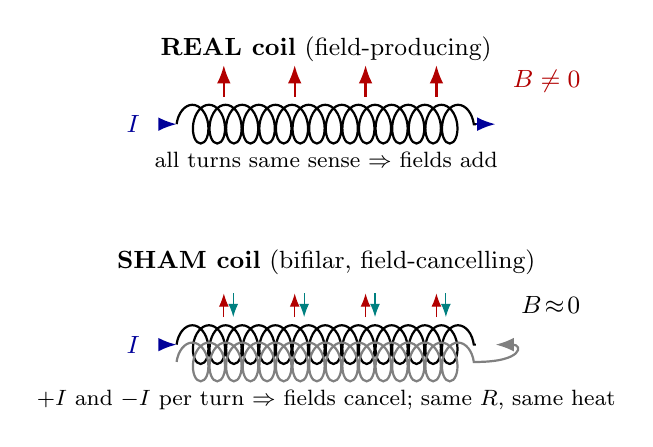
\begin{tikzpicture}[>=Latex,scale=1.0]
% --- REAL coil ---
\node at (2.1,2.35) {\small\textbf{REAL coil} (field-producing)};
\draw[thick,decorate,decoration={coil,aspect=0.6,segment length=6pt,
  amplitude=7pt}] (0.2,1.4) -- (4.0,1.4);
\draw[->,thick,blue!60!black] (0.0,1.4) -- (0.2,1.4);
\node[blue!60!black] at (-0.35,1.4) {\small $I$};
\draw[->,thick,blue!60!black] (4.0,1.4) -- (4.25,1.4);
% all turns same sense -> field up
\foreach \x in {0.8,1.7,2.6,3.5} \draw[->,red!70!black,thick]
   (\x,1.75) -- (\x,2.15);
\node[red!70!black] at (4.9,1.95) {\small $B\neq0$};
\node at (2.1,0.95) {\footnotesize all turns same sense $\Rightarrow$ fields add};

% --- SHAM coil ---
\node at (2.1,-0.35) {\small\textbf{SHAM coil} (bifilar, field-cancelling)};
\draw[thick,decorate,decoration={coil,aspect=0.6,segment length=6pt,
  amplitude=7pt}] (0.2,-1.4) -- (4.0,-1.4);
\draw[thick,decorate,decoration={coil,aspect=0.6,segment length=6pt,
  amplitude=7pt},gray] (0.2,-1.62) -- (4.0,-1.62);
\draw[->,thick,blue!60!black] (0.0,-1.4) -- (0.2,-1.4);
\node[blue!60!black] at (-0.35,-1.4) {\small $I$};
% wire 2 returns
\draw[->,thick,gray] (4.0,-1.62) .. controls (4.6,-1.62) and (4.6,-1.4) ..
   (4.25,-1.4);
% opposing arrows cancel
\foreach \x in {0.8,1.7,2.6,3.5}{
  \draw[->,red!70!black] (\x,-1.05) -- (\x,-0.75);
  \draw[->,teal] (\x+0.12,-0.75) -- (\x+0.12,-1.05);}
\node at (4.95,-0.9) {\small $B\!\approx\!0$};
\node at (2.1,-2.1) {\footnotesize $+I$ and $-I$ per turn $\Rightarrow$ fields cancel; same $R$, same heat};
\end{tikzpicture}
\caption{Real vs sham winding. Both use identical wire, turns and former;
the sham is wound bifilar (two wires together, connected to counter-run
the current) so its field cancels while its resistance and heating match
the real coil---the control that separates a genuine field effect from
placebo or coil-warming artifacts.}
\label{fig:bifilar}
\end{figure}

\noindent\textbf{Winding recipe (per coil).} (1)~Cut two equal wire
lengths ($\approx95$~m each for $R=15$~cm, $N=100$). (2)~Twist the two
starts together loosely and wind them \emph{as a pair}, $N$ turns, onto the
former---this is the bifilar layer. (3)~At the finish, join the end of
wire~1 to the end of wire~2 (the ``U-turn''); the two free starts become
the terminals. Current now flows out wire~1 through all turns and back
wire~2 through the same turns: net field $\approx0$, resistance $=2\times$
one-wire (identical to the real coil's series winding). Verify with the
gaussmeter: the sham should read $<0.05$~mT at the same current that gives
$1$~mT on the real coil.

\section{Bill of materials}
Table~\ref{tab:bom} is a realistic parts list (prices as of 2026, RU
retail, order of magnitude; reuse of a bench supply and an HRV device you
already own cuts the total substantially). A full new build is
$\sim\!12\,000$--$18\,000$~RUB; the minimum functional build
(reusing PSU + phone/watch HRV) is $\sim\!5\,000$~RUB.

\begin{table}[h]
\centering\small
\begin{tabular}{lllr}
\toprule
Item & Spec & Purpose & Price [RUB]\\
\midrule
Enamelled Cu wire & AWG20 (0.8 mm), $\ge400$ m & real + sham coils & 2\,000--3\,000\\
Coil formers ($\times2$) & 30 cm dia. ring (PVC/plywood/3D-print) & winding support & 500--1\,200\\
Constant-current driver & buck CC-CV, $\ge5$ A (XL4015 / DPS-class) & set-point field control & 500--900\\
DC supply & 12 V, $\ge10$ A (or reuse) & power & 0--3\,000\\
Linear Hall sensor & $\pm10$ mT ratiometric (or SS49E) & field calibration & 300--700\\
Microcontroller & Arduino Nano / ESP32 & current set-point, logging & 400--900\\
NTC + comparator & 45\,$^\circ$C cutout & thermal safety & 200--400\\
Relay/DPDT switch & coded real/sham selection & blinding & 300--600\\
Enclosure + connectors & --- & assembly & 800--1\,500\\
Thermal pad/insulation & limb-side & comfort/safety & 300--500\\
\midrule
\multicolumn{3}{l}{\textbf{Core electronics + coils subtotal}} & \textbf{5\,600--13\,100}\\
\addlinespace
HRV sensor & chest strap (Polar H10) or ring & recovery read-out & 0--7\,000\\
CK point-of-care (opt.) & finger-prick strips & muscle-damage marker & 0--3\,000\\
Dynamometer/jump mat (opt.) & grip or CMJ & force recovery & 0--4\,000\\
\bottomrule
\end{tabular}
\caption{Bill of materials. ``0'' entries are items commonly already owned
(bench supply, a watch/ring with HRV). Gaussmeter calibration can also use
a borrowed instrument.}
\label{tab:bom}
\end{table}

\section{Why ``less ROS'' is not automatically ``better recovery''}
\label{sec:hormesis}
Exercise-induced superoxide and $\text{H}_2\text{O}_2$ are
\emph{signalling} molecules: the acute burst drives mitochondrial
biogenesis, endogenous antioxidant upregulation and the training
adaptation itself (redox hormesis). Randomized trials show that blunting
this burst with high-dose vitamin~C/E can \emph{impair} endurance
adaptation and insulin sensitivity~\cite{ristow,gomez}. Consequences for
this instrument:
\begin{itemize}\itemsep2pt
\item a device that simply lowers ROS could \emph{reduce} training gains;
\item the plausible useful window is trimming a \emph{pathological excess}
  (acute injury, overtraining, ischaemia-reperfusion) while sparing the
  adaptive signal---an open question the instrument is built to test;
\item the right primary endpoint is therefore recovery \emph{without}
  degraded adaptation over weeks, not acute ROS alone.
\end{itemize}

\section{What a result would mean}
A reproducible, dose-shaped, sham-beating shift in a recovery read-out
would be the first human-level evidence that CISS-tuned radical-pair spin
chemistry is a controllable lever on exercise physiology---publishable
regardless of sign. A null result across the $0.2$--$3$~mT scan would bound
the in-vivo effect below the few-percent model prediction, which is itself
a useful, honest constraint. Either way the value is data, obtained with a
verified field and a blinded control---the opposite of the peak-reading,
uncalibrated ``free-energy'' tradition this project deliberately left
behind.

\begin{thebibliography}{9}\small
\bibitem{cisspaper} O.~Kirichenko, ``Chirality-induced spin selectivity as
  a spin gate on mitochondrial superoxide production: a radical-pair
  model,'' companion note (this folder).
\bibitem{usselman} R.~J.~Usselman \emph{et al.}, ``The quantum biology of
  reactive oxygen species partitioning impacts cellular bioenergetics,''
  Sci.\ Rep.\ \textbf{6} (2016) 38543.
\bibitem{ristow} M.~Ristow \emph{et al.}, ``Antioxidants prevent
  health-promoting effects of physical exercise in humans,'' PNAS
  \textbf{106} (2009) 8665.
\bibitem{gomez} M.~C.~Gomez-Cabrera \emph{et al.}, ``Oral administration of
  vitamin~C decreases muscle mitochondrial biogenesis and hampers
  training-induced adaptations in endurance performance,'' Am.\ J.\ Clin.\
  Nutr.\ \textbf{87} (2008) 142.
\end{thebibliography}

\end{document}
